\documentclass[twocolumn]{aastex631}

\usepackage{blindtext}

\newcommand{\tess}{\textit{TESS}}
\newcommand{\sname}{V1298~Tau}
\newcommand{\allplanets}{V1298~Tau~bcd}
\newcommand{\planetb}{V1298~Tau~b}
\newcommand{\planetc}{V1298~Tau~c}
\newcommand{\planetd}{V1298~Tau~d}
\newcommand{\planete}{V1298~Tau~e}
\newcommand{\rearth}{$R_\oplus$}
\newcommand{\exoplanet}{\texttt{exoplanet}}



\begin{document}

\title{Updated Ephemerides of the young multi-planet system V1298 Tau from TESS}

\author[0000-0002-9464-8101]{Adina~D.~Feinstein}
\altaffiliation{NSF Graduate Research Fellow}
\affiliation{Department of Astronomy and Astrophysics, University of Chicago, Chicago, IL 60637, USA}

\author[0000-0001-6534-6246]{Trevor J.\ David}
\affiliation{Center for Computational Astrophysics, Flatiron Institute, New York, NY 10010, USA}
\affiliation{Department of Astrophysics, American Museum of Natural History, New York, NY 10024, USA}

\author{Charles Beichman}
\affiliation{Caltech/IPAC, 1200 E. California Blvd. Pasadena, CA 91125, USA}


\author[0000-0002-3199-2888]{Sarah Blunt}
\altaffiliation{NSF Graduate Research Fellow}
\affiliation{Department of Astronomy, California Institute of Technology, Pasadena, CA, USA}


\author[0000-0002-4881-3620]{John~H.~Livingston}
\affiliation{Department of Astronomy, University of Tokyo, 7-3-1 Hongo, Bunkyo-ku, Tokyo 113-0033, Japan}

\author[0000-0001-7516-8308]{Benjamin~T.~Montet}
\affiliation{School of Physics, University of New South Wales, Sydney, NSW 2052, Australia}
\affiliation{UNSW Data Science Hub, University of New South Wales, Sydney, NSW 2052, Australia}

\author{DFM?}

\correspondingauthor{Adina~D.~Feinstein;\\ \twitter{afeinstein20}; \github{afeinstein20};} \email{afeinstein@uchicago.edu} 

%%%%%%%%%%%%%%%%%%%%
% abstract must be < 250 words
% currently at 180 words
%%%%%%%%%%%%%%%%%%%%
\begin{abstract}
\sname is a young ($\sim$23~Myr) solar analogue hosting four transiting exoplanets. Given its planets range between 0.5 - 0.9 $R_J$, this system provides a unique opportunity to understand the evolution of planetary radii in the same stellar environment. \sname was originally observed 6 years ago during K2 Campaign 4. The extended mission of NASA's Transiting Exoplanet Survey Satellite (\tess) includes observing the ecliptic plane. Here, we present new photometric observations of \sname from the 10-minute TESS Full-Frame Images. We use the TESS data to update the transit-timing for \allplanets as well as compare newly observed radii to that derived from the K2 light curve. We additionally catch a transit of \planete, which was a single-transit event in the previous data, allowing us to further constrain the period of this farthest known planet. \sname is the target of several ongoing and future observations, including with the James Webb Space Telescope. These updated ephemerides will be crucial for accurately recovering transit events and understanding any future doppler tomographic or transmission spectroscopy signals.\end{abstract}

%%%%%%%%%%%%%%%%%%%%

\keywords{Exoplanets (498) --- Pre-main sequence (1289) --- Starspots (1572) --- Stellar activity (1580)}

%%%%%%%%%%%%%%%%%%%%

\section{Introduction} \label{sec:intro}
Planetary sizes are expected to evolve over time, due to a variety of endogenous and exogenous physical processes including gravitational contraction, atmospheric heating and mass-loss, and core-envelope interactions \citep[e.g.][]{OwenWu2013, Lopez2013, Jin2014, ChenRogers2016, Ginzburg2018}. Dramatic size evolution is expected at early stages, when planets are still contracting and radiating away the energy from their formation, and when host stars are heating planetary atmospheres with high levels of X-ray and ultraviolet radiation. Since the size evolution of any individual planet is believed to be slow relative to typical observational baselines, the best way to make inferences about the size evolution of exoplanets is by measuring the sizes of large numbers of planets across a range of ages. 

NASA's Transiting Exoplanet Survey Satellite \citep[TESS,][]{Ricker2015} has made significant inroads toward this objective. \tess's observations of $\sim 90 \%$ of the sky have allowed for exoplanet transit searches around stars ranging from the pre-main sequence to the giant branch. It is through targeted surveys of young stars such as the THYME \citep[e.g.][]{Newton2019}, PATHOS \citep[e.g.][]{Nardiello2020}, and CDIPS \citep[e.g.][]{Bouma2020} surveys, along with case studies of individual systems \citep[e.g.][]{benatti19, Plavchan2020, Hedges2021, Zhou2021} that the timeline for planetary radius evolution can be pieced together. 

The \sname planetary system is one particularly valuable benchmark for understanding the size evolution of exoplanets. \sname is a pre-main sequence, approximately solar-mass star that was observed in 2015 by NASA's \textit{K2} mission \citep{Howell2014}. Analysis of the \textit{K2} data revealed the presence of four transiting planets, all with sizes between the sizes of Neptune and Jupiter \citep{David2019a, David2019b}. There are no other known examples of exoplanetary systems with so many planets larger than Neptune interior to 0.5~au, despite the high completeness of the Kepler survey to large ($>5$~\rearth), close-in planets. This observation raises the possibility of a causal connection between the extreme youth of \sname and the uncommonly large sizes of its planets.  

The youth of \sname was initially established on the basis of its strong X-ray emission \citep{Wichmann1996} and high photospheric lithium abundance \citep{Wichmann2000}. An analysis of Gaia DR1 astronometric data found \sname was co-moving with 8 other stars \citep[Group 29;]{Oh2017} and derived an age of $\sim 40$~Myr \citep{Luhman2018}. However, more recent analyses based on Gaia EDR3 astrometry suggests \sname belongs to either the D2 or D3 subgroups of Taurus, both of which have estimates ages $\lesssim$10~Myr \citep[][Gaidos et al. submitted]{Krolikowski2021}. Other studies focused specifically on the \sname system have estimated its age to be 23$\pm$4~Myr from comparison with empirical and theoretical isochrones \citep{David2019b}, or 28$\pm$4~Myr from isochrone fitting to the \citet{Luhman2018} Group 29 membership list given Gaia EDR3 data (Johnson et al. submitted).

%An analysis of the Gaia DR1 astrometric data found that \sname was co-moving with 8 other stars \citep{Oh2017}. \citet{Luhman2018} used Gaia DR2 astrometry to expand the membership of this group, referred to as Oh's Group 29, and examine its relationship to the Taurus-Auriga star-forming region. \citet{Luhman2018} concluded that while Group 29 is indeed young ($\sim$40~Myr), the collection of stars was physically unrelated to the traditional star-forming groups within the Taurus-Auriga complex.  

Given the system's youth and potential to reveal information about the initial conditions of close-in planetary systems, \sname has been the target for extensive follow-up observations. These include efforts to constrain planet masses with radial velocities \citep{Beichman2019}, measure the spin-orbit alignments of planet c \citep{Feinstein21} and planet b (Johnson et al. submitted; Gaidos et al. submitted), measure or constrain atmospheric mass-loss rates for the innermost planets \citep{Schlawin21, Vissapragada21}, and an approved program to study the planetary atmospheres using the James Webb Space Telescope \citep{Desert2021}.


Here we report on newly acquired TESS observations of \sname which help to refine the orbital ephemerides of the transiting planets and enable comparison of the planet sizes inferred from two different telescopes with different bandpasses (\tess\ and Kepler). We describe the observations in Section~\ref{sec:observations}, our analysis procedures in Section~\ref{sec:analysis}, and our primary conclusions in Section~\ref{sec:conclusions}.

%%%%%%%%%%%%%%%%%%%%%%%%%%%%%%%%%%%%%%%%%%%%%%%%%%%%%%%
\begin{figure}[!ht]
\begin{center}
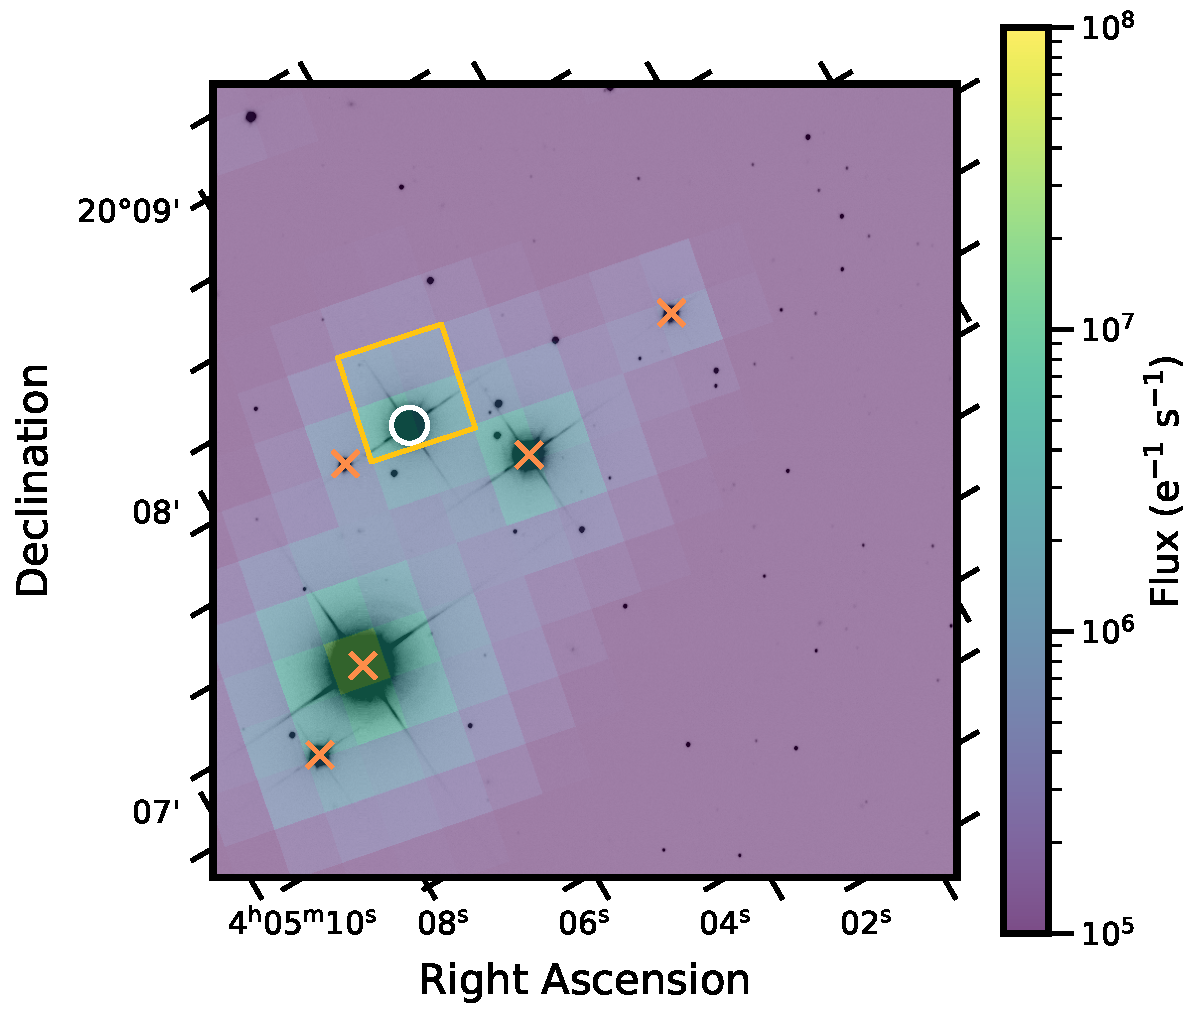
\includegraphics[width=0.46\textwidth,trim={0.25cm 0 0 0}]{static/TESSaperture.pdf}
\caption{The \tess\ target pixel file (TPF) overlaid with a sky image of \sname taken with the Sloan Digital Sky Survey (SDSS) i-band. \sname is shown in the white circle; nearby sources with \tess\ magnitudes $< 14$ are marked with orange x's. There are two bight nearby sources to \sname. However, selecting the one pixel aperture (white square) encapsulates only \sname and therefore contamination from the nearby sources is negligible. \label{fig:tpf}}
\end{center}
\end{figure}
%%%%%%%%%%%%%%%%%%%%%%%%%%%%%%%%%%%%%%%%%%%%%%%%%%%%%%%

\section{TESS Observations} \label{sec:observations}

During its Extended Mission Cycle 4, \tess\ is re-observing many of the previous \textit{K2} fields. \sname (TIC 15756231) was observed by \tess\ in Sectors 43 (UT 16 Sep 2021 to UT 12 Oct 2021) at 10-minute cadence within the Full-Frame Images (FFIs). We used the \texttt{tica} \citep{fausnaugh20} software to download calibrated FFIs each orbit for Sectors 43, as these FFIs are quickly available after the data is down-linked. We created light curves from the \texttt{tica}-processed FFIs by modeling the point-spread function (PSF) of \sname and the two nearby bright sources (see Figure~\ref{fig:tpf}). While aperture photometry provided a decent light curve, we found that modeling each star (3 in total) with a 2D Gaussian created a less contaminated light curve for \sname (Figure~\ref{fig:transits}, top row). %This allowed us to place initial constraints on the planets' ephemerides. The remaining analysis was completed using the SPOC-processed light curves.




%%%%%%%%%%%%%%%%%%%%%%%%%%%%%%%%%%%%%%%%%%%%%%%%%%%%%%%
\begin{figure*}[!ht]
\begin{center}
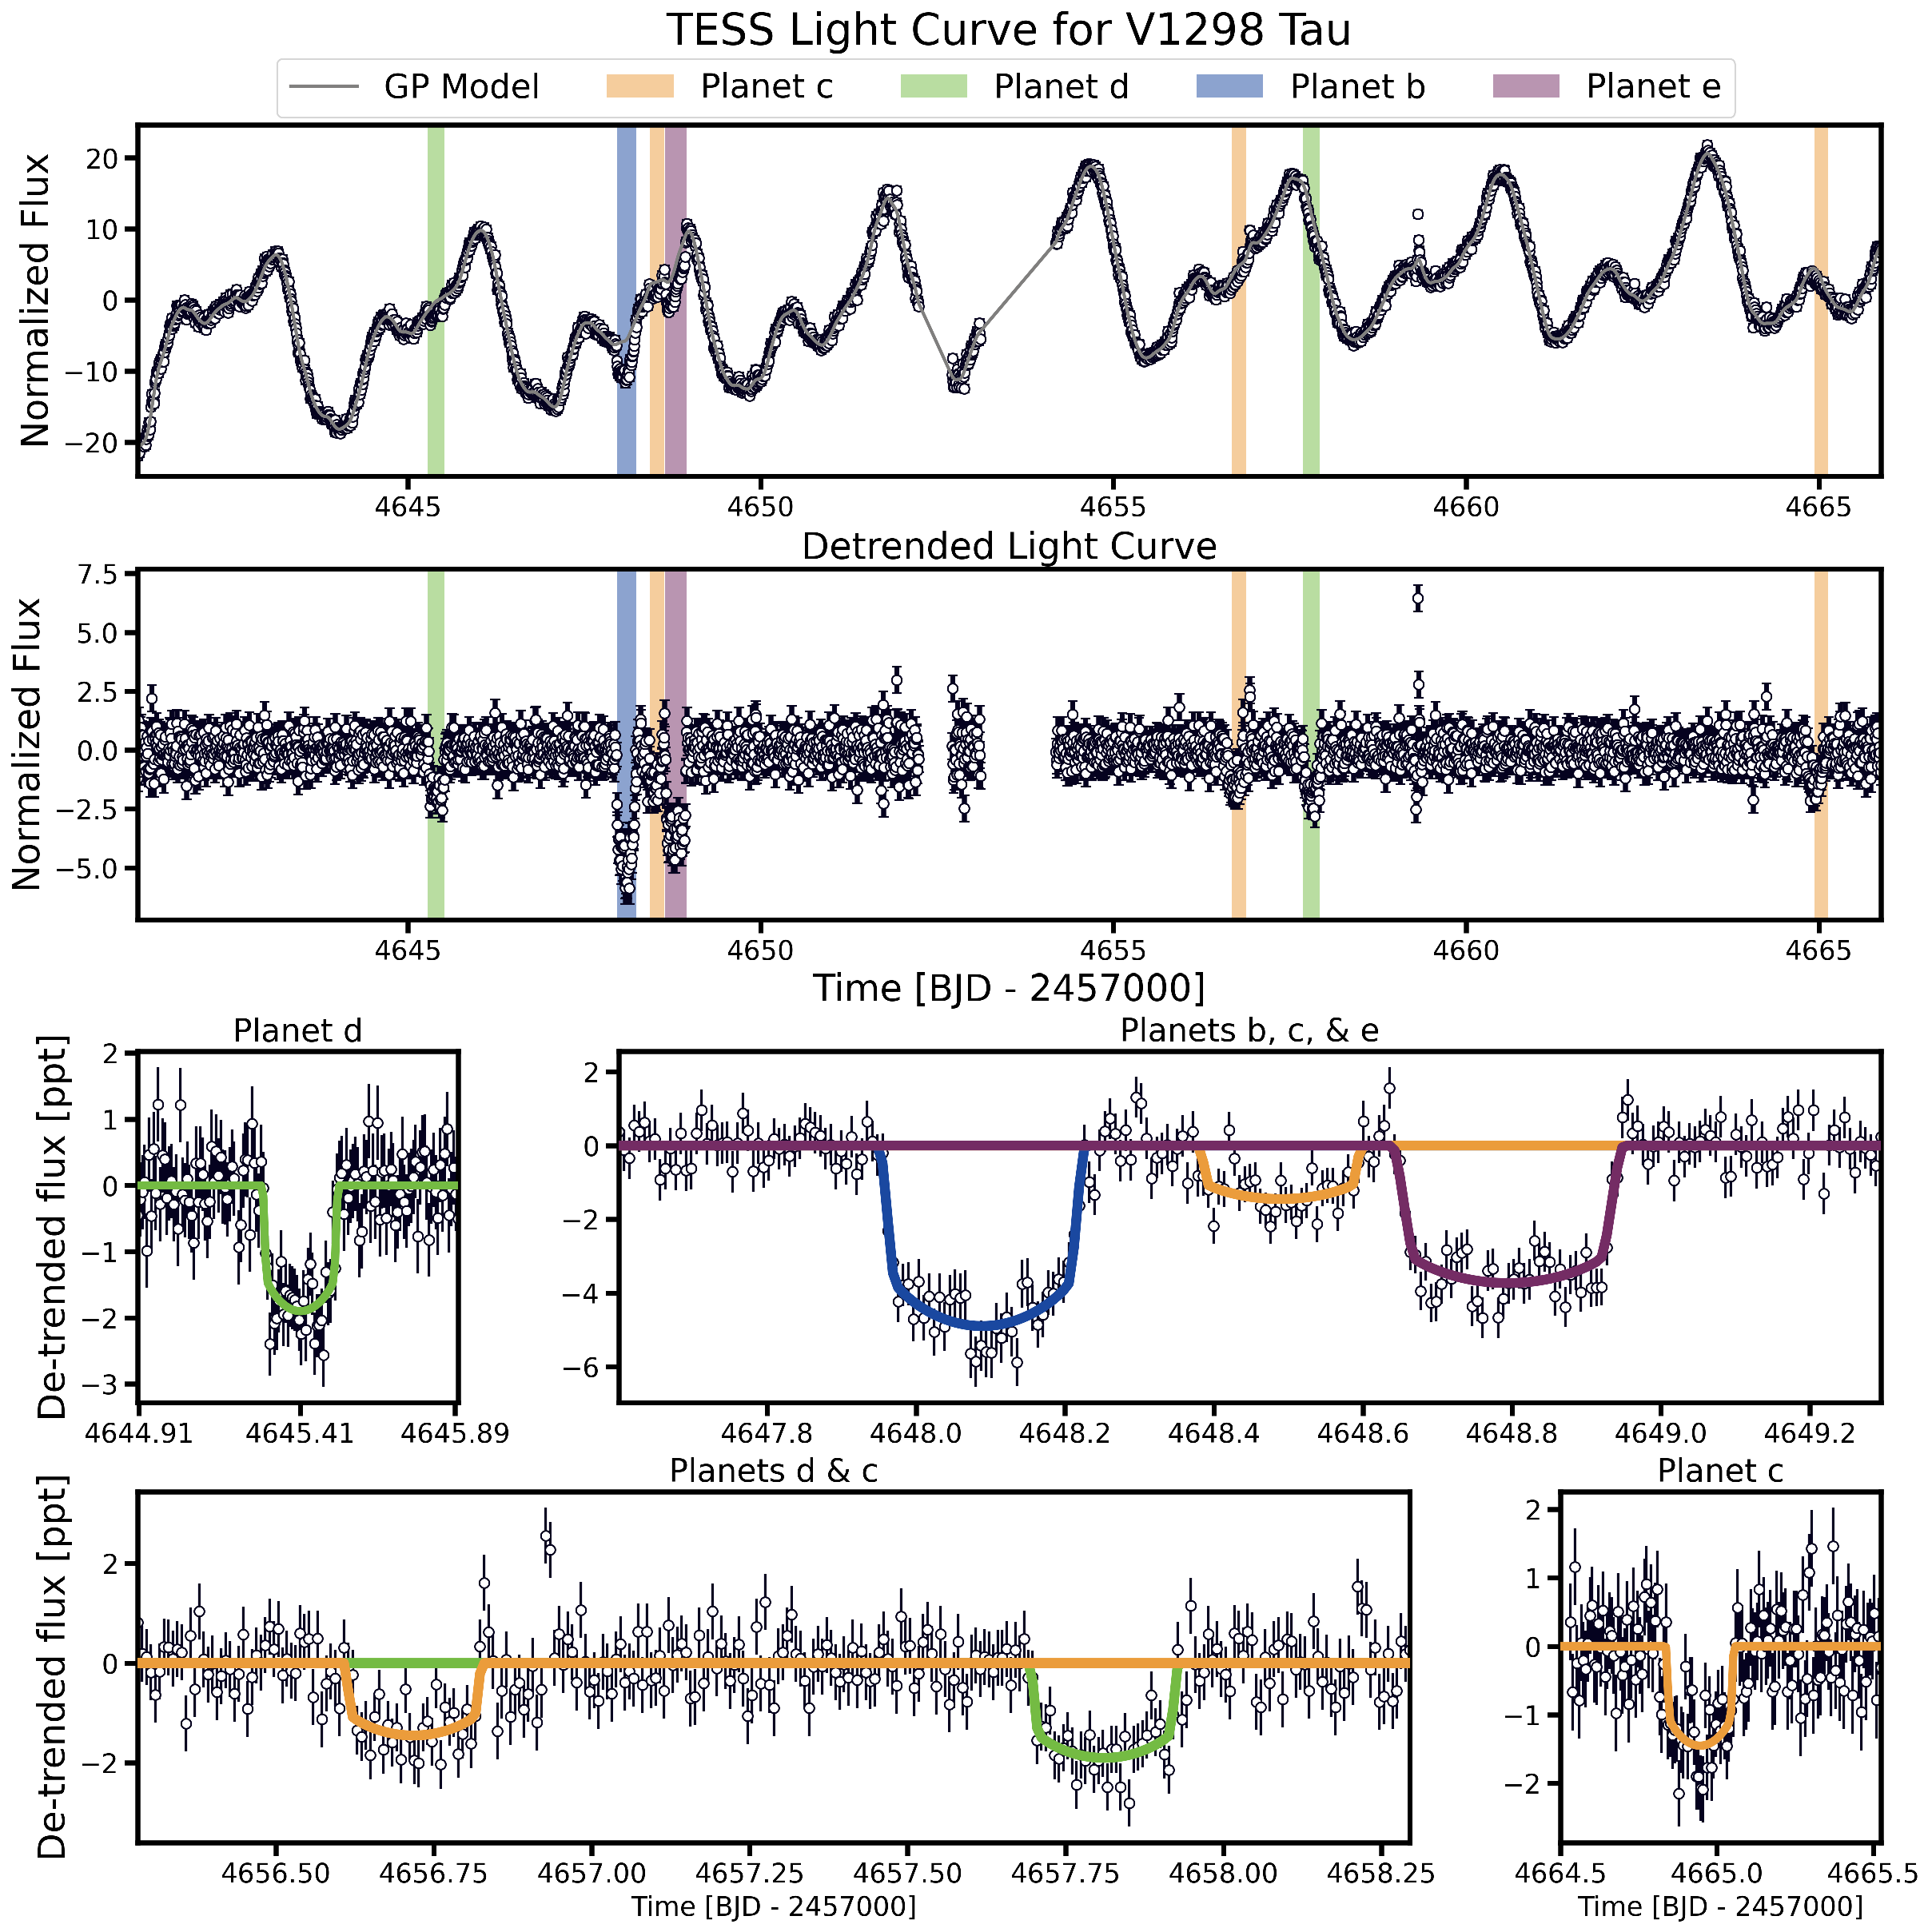
\includegraphics[width=\textwidth,trim={0.25cm 0 0 0}]{static/lightcurve.pdf}
\caption{\sname extracted light curve from the \texttt{tica}-processed full-frame images, with transits of \allplanets highlighted by color. Top row: extracted light curve with over plotted with our best-fit GP model for stellar variability (blue). Middle row: the \tess\ light curve with the stellar variability removed by our model. Bottom rows: zoomed-in regions around the visible transits during the first orbit (third row) and second orbit (last row) from \tess\ Sector 43. \label{fig:transits}}
\end{center}
\end{figure*}
%%%%%%%%%%%%%%%%%%%%%%%%%%%%%%%%%%%%%%%%%%%%%%%%%%%%%%%


%%%%%%%%%%%%%%%%%%%%%%%%%%%%%%%%%%%%%%%%%%%%%%%%%%%%%%%
\begin{figure}[!ht]
\begin{center}
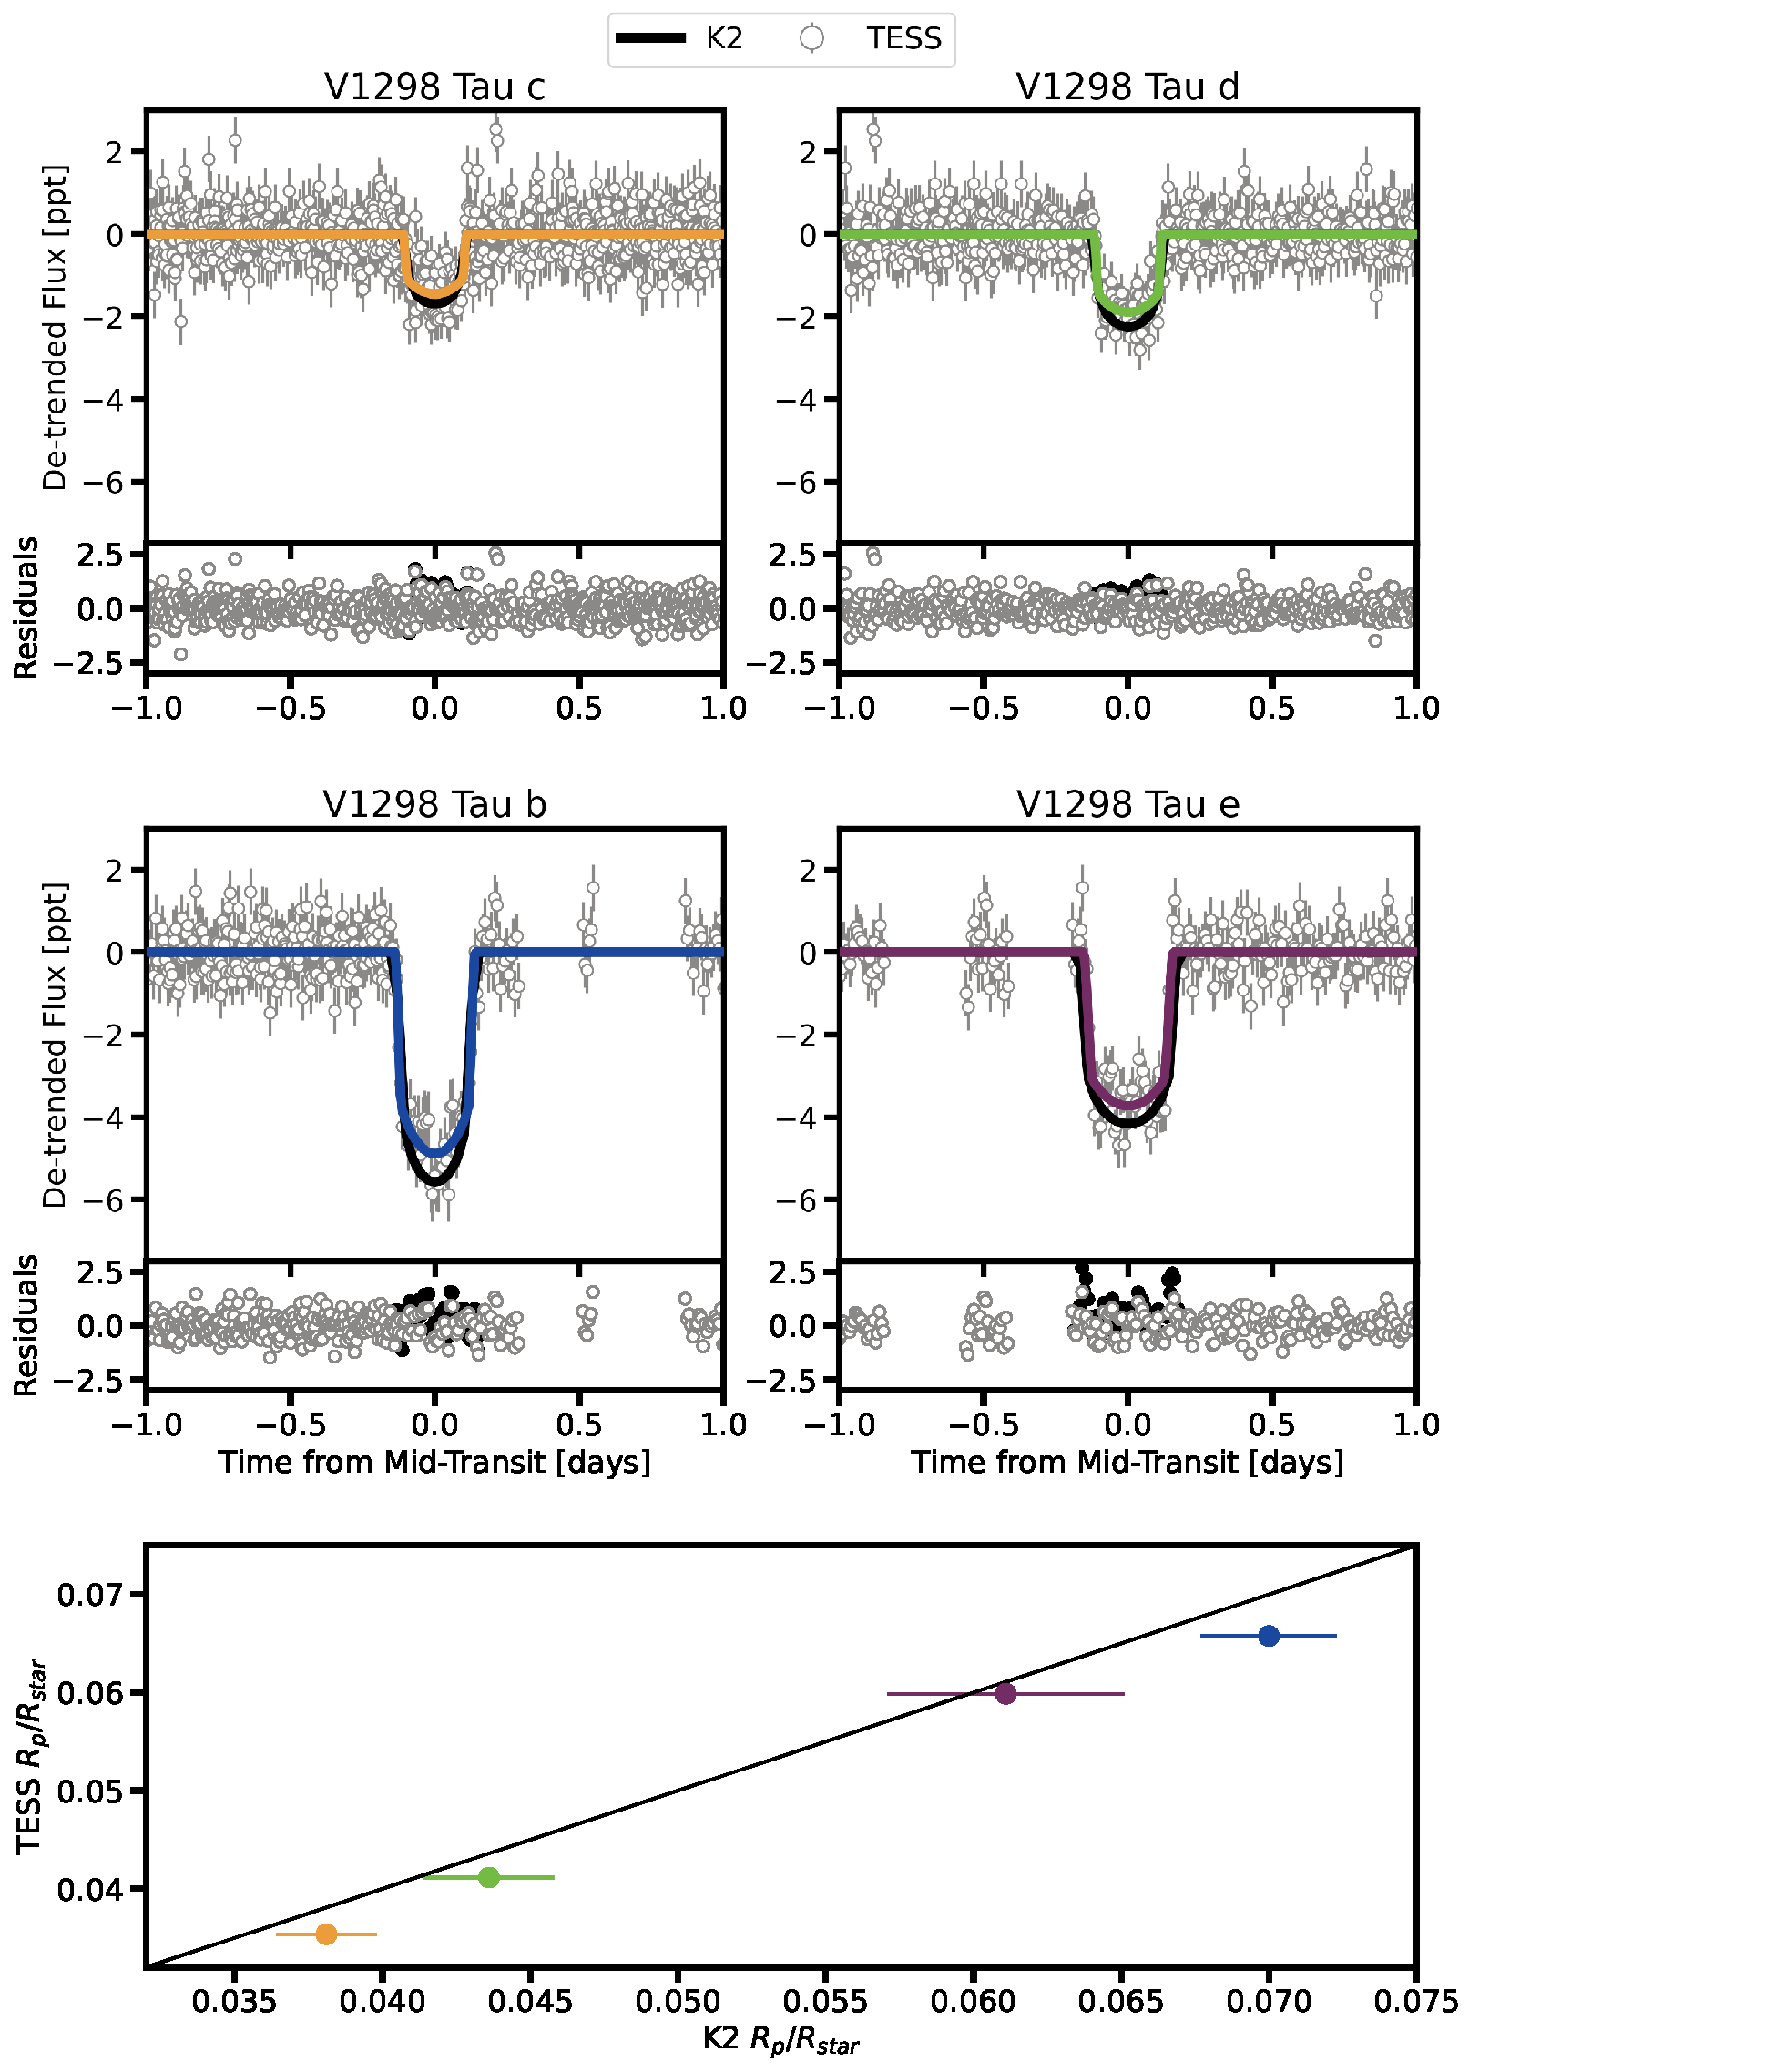
\includegraphics[width=0.465\textwidth,trim={0.25cm 0 4.5cm 0}]{static/folded_compare.pdf}
\caption{Phase-folded \tess\ data (gray) with the new best-fit model (color) compared to the best-fit parameters from the original \textit{K2} data (black). The residuals between the data and each fit are shown underneath. A comparison of measured $R_p/R_\star$ are presented at the bottom, with a 1-to-1 line plotted in black for reference. The transit depth from the \textit{K2} data is deeper than that from \tess, particularly for \planetb and \planete. \label{fig:compare}}
\end{center}
\end{figure}
%%%%%%%%%%%%%%%%%%%%%%%%%%%%%%%%%%%%%%%%%%%%%%%%%%%%%%%

\section{Analysis} \label{sec:analysis}

% planet fits
We simultaneously modeled the transits of \allplanets and the stellar variability using the open-source packages \exoplanet \citep{exoplanet2019, exoplanet2021} and \texttt{PyMC3} \citep{Salvatier16}. Transit timings were originally identified using updated ephemerides from \textit{Spitzer} (Livingston et al. in prep). All other transit parameters (presented in Table~\ref{tab:table}) were initialized using values from \cite{David2019a}. We assumed quadratic limb darkening law, following the reparameterization described by \cite{kipping13}; this method allows for an efficient and uniform sampling of limb-darkening fits.

% light curve fits

Since the \texttt{tica} FFIs do not provide an error estimate, we fit for flux errors within our GP model. We define the flux error as

\begin{equation}
    \sigma_y = e^{ln(\sigma_l)} + y^2 e^{2 ln(\sigma_j)}
\end{equation}

where $y$ is the flux array, and $\sigma_l$  and $\sigma_j$ are used to define the light curve noise and in-transit jitter. $\sigma_l$  and $\sigma_j$ are also used as the first and second terms in our rotation model, which we defined as a stochastically-driven, damped harmonic oscillator, defined by the \texttt{SHOTerm} in \texttt{celerite} \citep{dfm17}.

We took a two-step approach to modeling any background contamination. First, we defined a quadratic trend with respect to time for varying the background flux, where each term was drawn from a normal distribution (listed as `trend term' in Table~\ref{tab:table}). Then, we generated a Vandermonde matrix ($A$) of time. This is a way of introducing a polynomial least-squares regression with respect to time. The final background flux was calculated by taking $bkg = A \cdot trend$.  

\section{Discussion} \label{sec:discussion}



\subsection{\textit{K2} vs. \tess}

We compare the differences in transit parameters between the \textit{K2} and \tess\ data in Figure~\ref{fig:compare}. We plot the best-fit transit model from \textit{K2} in black, which was generated using parameters from \cite{David2019a} and the \texttt{batman} transit-modeling software \citep{Kreidberg15}. It is important to note that the \textit{K2} bandpass ranges from $\sim 400-900$~nm \citep{Howell2014}, while the \tess\ bandpass ranges from $\sim 600-1000$~nm \citep{Ricker2015}.


\subsection{Constraining \planete's Period}

There was a single transit of \planete in the original \textit{K2} data, which occurred roughly in the middle of the campaign. Since no other transits were detected, this provides a lower period limit of 36~days. 



\section{Conclusions} \label{sec:conclusions}

We present new ephemerides for all four known planets in the \sname system. We have recovered the second transit of \planete; this new transit time in combination from the transit observed with \textit{K2} has allowed us to place tighter constraints on the period of the outermost planet.

A full transit-timing variation (TTV) analysis using \textit{K2}, \textit{Spitzer}, and \tess\ ephemerides is presented in Livingston et al. (in prep).



The Python code used to access the data, process and model the light curve, and reproduce the tables and figures are made publicly available.\footnote{\url{https://github.com/afeinstein20/v1298tau_tess}}


\begin{deluxetable*}{l r r r r}[!ht]
\tabletypesize{\footnotesize}
\tablecaption{\sname light curve fitting results. \label{tab:table}}
\tablehead{\\
\hline\
\textit{Star} & \textit{Value} & \textit{Prior} &  & \\
\hline
$R_\star [R_\odot]$ & & $\mathcal{G}(1.305, 0.07)$ & & \\
$u_1$ & & & & \\
$u_2$ & & & & \\
$P_{rot}$ [days] & & $\mathcal{G}($ln$ 2.87, 2)$ & & \\
ln($A$ [ppt]) & & & & \\
ln($Q_0$) & & $\mathcal{H}(\sigma=2)$ & & \\
$\Delta Q_0$ & & $\mathcal{G}(0, 2)$ & & \\
$\rho_\textrm{SHO}$ & & $\mathcal{G}(0, 10)$ & & \\
$\sigma_\textrm{SHO}$ & & $\mathcal{G}(\sigma_\textrm{flux}, 10)$ & & \\
f [ppt] & & & & \\
mix & & & & \\
\hline\
\textit{Light Curve} & \textit{Value} & \textit{Prior} &  & \\
\hline
trend term a & & $\mathcal{G}(0, 0.01)$ & & \\
trend term b & & $\mathcal{G}(0, 0.1)$ & & \\
trend term c & & $\mathcal{G}(0, 1)$ & & \\
$\sigma_l$ & & $\mathcal{G}($ln$(0.1\sigma_\textrm{flux}), 10)$  & & \\
$\sigma_j$ & & $\mathcal{G}($ln$(0.1\sigma_\textrm{flux}), 10)$  & & \\
\hline\
\textit{Planets} & \textit{c} & \textit{d} & \textit{b} & \textit{e}\\
\hline
P [days]               &  &  &  &  \\
$T_0$ [BJD - 2457000]  &  &  &  &  \\
Depth [ppt]            &  &  &  &  \\
$R_p/R_\star$          &  &  &  &  \\
$a/R_\star$            &  &  &  &  \\
$b$                    &  &  &  &  \\
$e$ [$^\circ$]         &  &  &  &  \\
\hline\
\textit{Priors} & \textit{c} & \textit{d} & \textit{b} & \textit{e}\\
\hline
log($P$ [days]) & $\mathcal{G}($ln$ 8.25, 1)$ & $\mathcal{G}($ln$ 12.40, 1)$& $\mathcal{G}($ln$ 24.14, 1)$ & $\mathcal{G}($ln$ 36.70, 1)$\\
$T_0$ [BJD - 2457000] & $\mathcal{G}(4648.53,0.1)$ & $\mathcal{G}(4645.4,0.1)$ & $\mathcal{G}(4648.1,0.1)$ & $\mathcal{G}(4648.8,0.1)$ \\
log(depth [ppt]) & $\mathcal{G}($ln$ 1.45, 1)$ & $\mathcal{G}($ln$ 1.90, 1)$ & $\mathcal{G}($ln$ 4.90, 1)$ & $\mathcal{G}($ln$ 3.73, 1)$ \\
$b$ & $\mathcal{U}[0, 1]$ & $\mathcal{U}[0, 1]$ & $\mathcal{U}[0, 1]$ & $\mathcal{U}[0, 1]$ \\
duration [days] & $\mathcal{G}($ln$ 0.19, 1)$ & $\mathcal{G}($ln$ 0.23, 1)$ & $\mathcal{G}($ln$ 0.27, 1)$ &  $\mathcal{G}($ln$ 0.31, 1)$
}
\startdata
\enddata
\tablecomments{Priors are noted for parameters that were directly sampled. The distributions are as follows -- $\mathcal{G}$: Gaussian; $\mathcal{H}$: Half-normal; $\mathcal{U}$: Uniform. $\sigma_\textrm{flux}$ is the standard deviation of the light curve}
\end{deluxetable*}

\begin{acknowledgments}
It is a pleasure to thank the Astronomical Data Group at the Flatiron Institute for helpful discussions. ADF acknowledges support from the National Science Foundation Graduate Research Fellowship Program under Grant No. (DGE-1746045).

This research has made use of NASA's Astrophysics Data System Bibliographic Services.
\end{acknowledgments}

\include{table}


%\vspace{5mm}
\facilities{TESS, Kepler}

\iffalse
\software{\texttt{exoplanet} \citep{exoplanet2021},
          \texttt{EVEREST 2.0} \citep{Luger2018},
          \texttt{K2SC} \citep{Aigrain2016},
          \texttt{K2PHOT} \citep{Petigura2018},
          \texttt{lightkurve} \citep{lightkurve},
          \texttt{lmfit} \citep{lmfit}, 
          \texttt{matplotlib} \citep{matplotlib},
          \texttt{PyMC3} \citep{exoplanet:pymc3},
          \texttt{starry} \citep{exoplanet:luger18},
          \texttt{theano} \citep{exoplanet:theano},
          \texttt{tica} \citep{fausnaugh20}
          }
\fi

\bibliography{main}{}
\bibliographystyle{aasjournal}


\end{document}
